\begin{frame}
{\textbf{Problem:6}\\A rectangular park is to be designed whose breadth is 3m less then its length. Its area is to be 4square metres more than the area of a park that already been made in the shape of an isosceles triangle with its base as the breadth of the rectangular park and of altitude of 12m. Find its length and breadth.}
\begin{itemize}
\item \textbf{Solution:}
\end{itemize}
\textbf{Given:} A rectangualr park \\
breadth = length - 3\\
A Isosceles triangle\\
Altitude = Height = 12m\\
Area of rectangle = Area of triangle + 4\\
base of the triangle = breadth of the rectangular  park.\\
\end{frame}
\begin{frame}
from the Given we need to find  lenght, breadth, Area$_{rec},$ Area$_{tri}$ ?\\
 Area of the rectangle
\begin{align}
 = l \times b
 \end{align}
= $l(l - 3).$\\
Area of the triangle
\begin{align}
 = \frac{1}{2} \times b \times h
\end{align}
 = $\frac{1}{2} \times (l -3)\times 12 = 6(l - 3).$\\
from the Given Area$_{rec}$ = Area$_{tri}$ + 4\\
i.e \enspace
$l(l - 3) = 6(l - 3) + 4$\\
$l^2 + 9l + 14 = 0$ \\
$l = 7.$\\
then, Area$_{tri}$ = 6(7 - 3) = 24 m$^2$\\
Area$_{rec}$ = 7 $\times$ 4 = 28 m$^2$ (or) Area$_{rec}$ =  24 + 4 = 28 m$^2.$\\
the python code for  Figure 1-11 is codes/tri\_rect.py\\
and the equivalent latex-tikz code for Figure 1-12 is fig/tri\_rect.tex
\end{frame}
\begin{frame}{}
\begin{figure}[!ht]
	\begin{center}
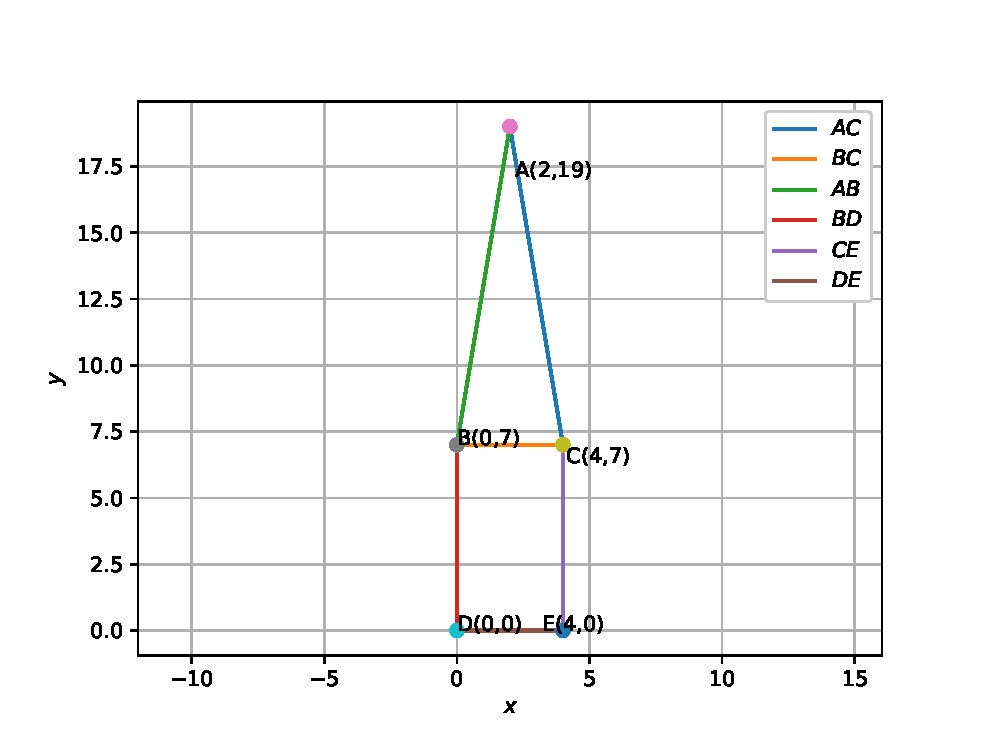
\includegraphics[width=1\columnwidth]{./figs/tri_rect.eps}
	\end{center}
	\caption{}
	\label{}	
\end{figure} 
\end{frame}
\begin{frame}{}
\begin{figure}[!ht]
	\begin{center}
		\resizebox{0.3\columnwidth}{!}{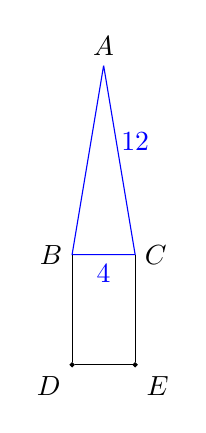
\begin{tikzpicture}
[scale=.2,>=stealth,point/.style={draw,circle,fill = black,inner sep=0.5pt},]

%Triangle sides
\def\a{4}
\def\b{7}
\def\c{3}
\def\d{2}
\def\e{19}

%Marking coordiantes
\color{black}
\coordinate [label=above:$A$] (A) at (\d,\e);
\coordinate [label=left:$B$] (B) at (0,\b);
\coordinate [label=right:$C$] (C) at (\a,\b);



%Drawing triangle ABC
\color{blue}
\draw (A) -- node[left] {$\textrm{}$} (B) -- node[below] {$\textrm{4}$} (C) -- node[above,,xshift=2mm] {$\textrm{12}$} (A);
\color{black}
\node (D) at (0, 0)[point,label=below left:$D$] {} ;
\node (E) at (\a, 0)[point,label=below right:$E$] {};

%Joining BD, CE and DE
\draw (B)--(D) ;
\draw (C)--(E);
\draw (D)--(E);

\end{tikzpicture}}
	\end{center}
	\caption{}
	\label{}	
\end{figure}
\end{frame}
\begin{frame}{}
\textbf{Coordinates:}
\begin{enumerate}
\item Take the point D as origin $\begin{pmatrix} 0\\0 \end{pmatrix}.$
\item E = $\begin{pmatrix} 4\\0 \end{pmatrix}.$
\item B = $\begin{pmatrix} 0\\7 \end{pmatrix}.$
\item Draw a line DB from the D to B.
\item C = $\begin{pmatrix} 4\\7 \end{pmatrix}.$
\item Join the all points of rectangle BCDE.\\
Then draw a triangle with the base of BC and with the altitude of A = 12.\\
\item A = $\begin{pmatrix} 2\\19 \end{pmatrix}.$
\item Join the all line segments of triangle ABC.  
\end{enumerate}
\end{frame}
\begin{frame}
\url{https://github.com/Narendrapulipati/geometry/blob/master/codes/tri_rect.py}
\url{https://github.com/Narendrapulipati/geometry/blob/master/figs/tri_rect.tex}
\end{frame}